\section{Non-laminar age group modeling}
With a full development of statistical rate models for a single age
group behind us, and many possibilities available, this section turns
to a peculiar feature of population rate meta-analysis: the wide
variety of age groups reported in the literature.

A typical example of the heterogeneity in age groups is shown in
Figure~\ref{theory-age_group_model-af_age_groups}.  The middle of the
age group is scattered against the width of the age group.  Simply
put, there is no standard set of age groups for epilepsy research, and
different studies use report results with different age groups.

\begin{figure}[h]
\begin{center}
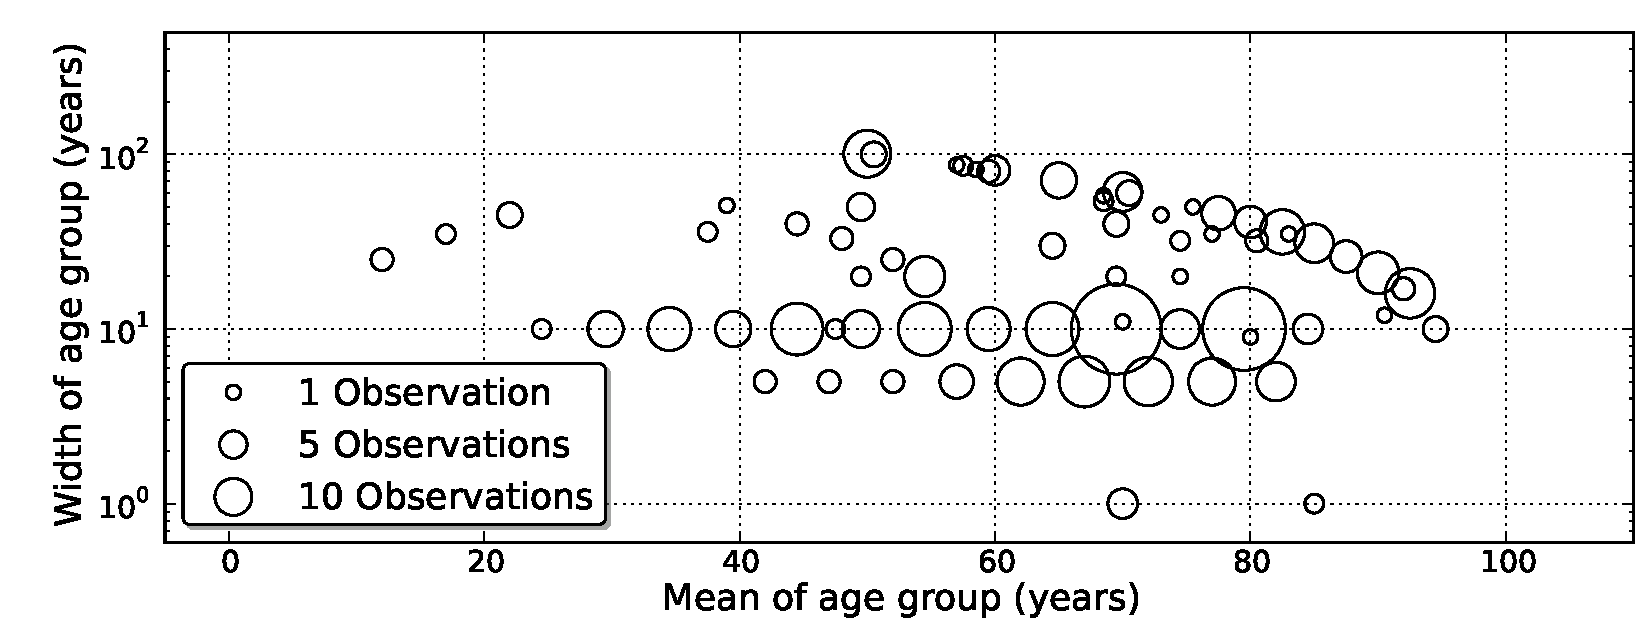
\includegraphics[width=\textwidth]{af_age_groups_scatter.png}
\end{center}
\caption{Mean and spread of age groups in the prevalence data collected
  from a systematic review of epilepsy (jittered to show density).
  There were $<<len(d['af_age_groups.json']['data'])>>$ rows of prevalence
  data extracted, but the most common age
  group accounted for only $<<d['af_age_groups.json']['most_freq_cnt']>>$ rows.}
\label{theory-age_group_model-af_age_groups}
\end{figure}

This variation in reporting would be no problem if I had access to the
microdata gathered in the course these studies.  From microdata, for
example from a national health information system or from a
demographic household survey, I could simply tally the prevalence
rates by single year age groups.  Although each individual row of data
gathered in this way would have high variability, the rate model from
the last section combined with the age pattern model would do their
work to come up with a combined estimate that is as uncertain as it
should be.

This approach is occassionally a possibility in a GBD study, and I
expect it to be possible more frequently when in national and
subnational settings.  In the unfortunate, but common, situation that
the rate microdata is not available, then the rates cannot be
re-tallied into homogeneous, appropriately fine age groups, and an
alternative approach is needed.

Discussion of typical approach, using the midpoint of the age range is
the level:
For example in print: \url{
  http://www.rachel.org/lib/meta_leukemias_near_nukes.070701.pdf }

